\def \MOISEp {$\mathcal{M}OISE^+$} 

\chapter{Methodology}
\label{ch:methodology}

In order to develop the new strategy for the team based on an organizational model, the entire workflow of the project was subdivided into several distinct phases. These phases include the initial phases of the project, one cycle of work related to the definition of the specification of the new strategy, another cycle related to the implementation of the strategy, and the final phases of the work, as depicted in Figure \ref{fig:methodology}.

The initial phases of the project consisted of two parts. The first phase of the work was to carry out an analysis of the feasibility of adopting the \MOISEp \cite{MOISEp} model to better understand the system and to observe how a new strategy could be implemented. This analysis will be presented in Chapter \ref{ch:target_system}. After that, before starting the development of the project, the requirements for its implementation were listed, as will be seen in Chapter \ref{ch:requirements}.

The project followed a development cycle consisting of two phases: specification and implementation. The development started with the specification cycle, in which several iterations of the specification were performed to refine the specifications until the first implementable version was achieved. Once the initial specification was finalized, the implementation cycle began, which started with the implementation of the tree nodes. Then, with all tree nodes implemented, the first implementation of the team's strategy BT was assembled. 

The implemented BT was then used to test the system against the FSM-based system to ensure that the new system performed at least as well and could cover the same use cases. Finally, the tested system was submitted for review by the ThunderVolt team; this review was then used to fix some problems with the specification of the tree, starting the specification cycle all over again, and in other cases to fix implementation errors, starting the implementation cycle all over again. After many tests and revisions, a final version of the implementation was obtained, which was then merged into the team's main code branch. 

The detailed specification and implementation of the tree structure will be presented in Chapter \ref{ch:development}, while the results of the performance tests comparing the BT-based system with the FSM-based system will be discussed in Chapter \ref{ch:results}.

After finishing the system improvements, all changes were validated in an academic competition, the \textit{IRONCup 2023} \cite{IRONCup2023}, and the results of the competition will also be shown in Chapter \ref{ch:results}.

\begin{figure}
    \centering
    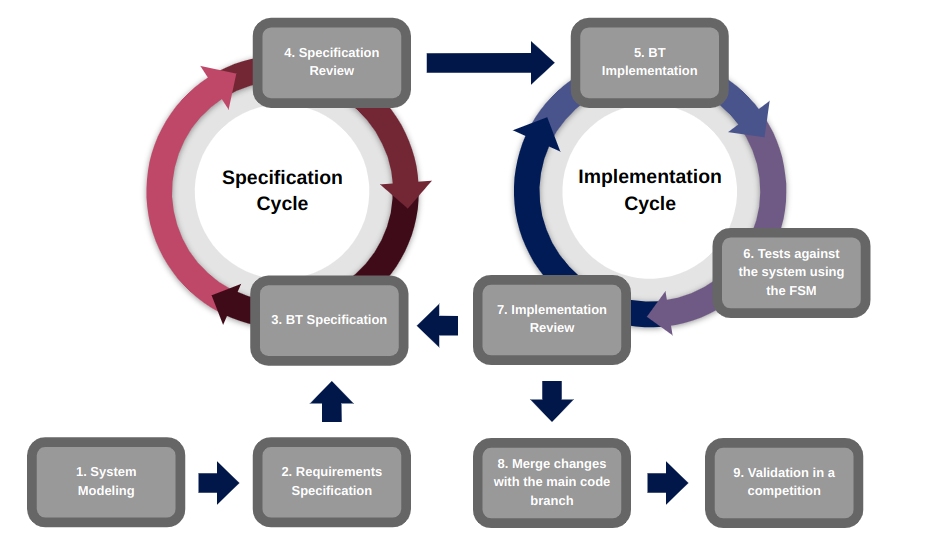
\includegraphics[width=\linewidth]{images/Methodology.png}
    \caption{Work methodology and development cycle}
    \label{fig:methodology}
\end{figure}
